\subsection{Turm}

Um den Aus- und Einlagerungsvorgang besser darzustellen sollte ein Modell des Turms gebaut werden. Dieser sollte den Aktuellen Status (belegte und ausgelagerte Stellplätze) des Turmes darstellen und auf Anfragen des Clients reagieren. Es sollte sozusagen ein Prototyp des Turmes entstehen, welcher die Funktionalität des Turmes simuliert. Mittels RGB LEDs sollten die Stellplätze des Turmes dargestellt werden.

Abgesehen von der Hardware, sollte der Turm auch Software beinhalten um sozusagen als Backend für die App zu dienen. Jeder Turm sollte als eigenständige Einheit dienen und Anfragen selbstständig beantworten können.

Da das Projektteam sowohl die 3D-Drucker der HTL, als auch einen eigenen 3D-Drucker zur Verfügung hatte, wurde entschieden, dass der Turm aus 3D-Druckteilen bestehen sollte. 3D-Druck erlaubt dem Projektteam, den Turm sehr schnell und ohne viel Aufwand zu bauen. Zudem kann der Turm auch Detailreicher gestaltet werden.

\begin{figure}[H]
  \centering
  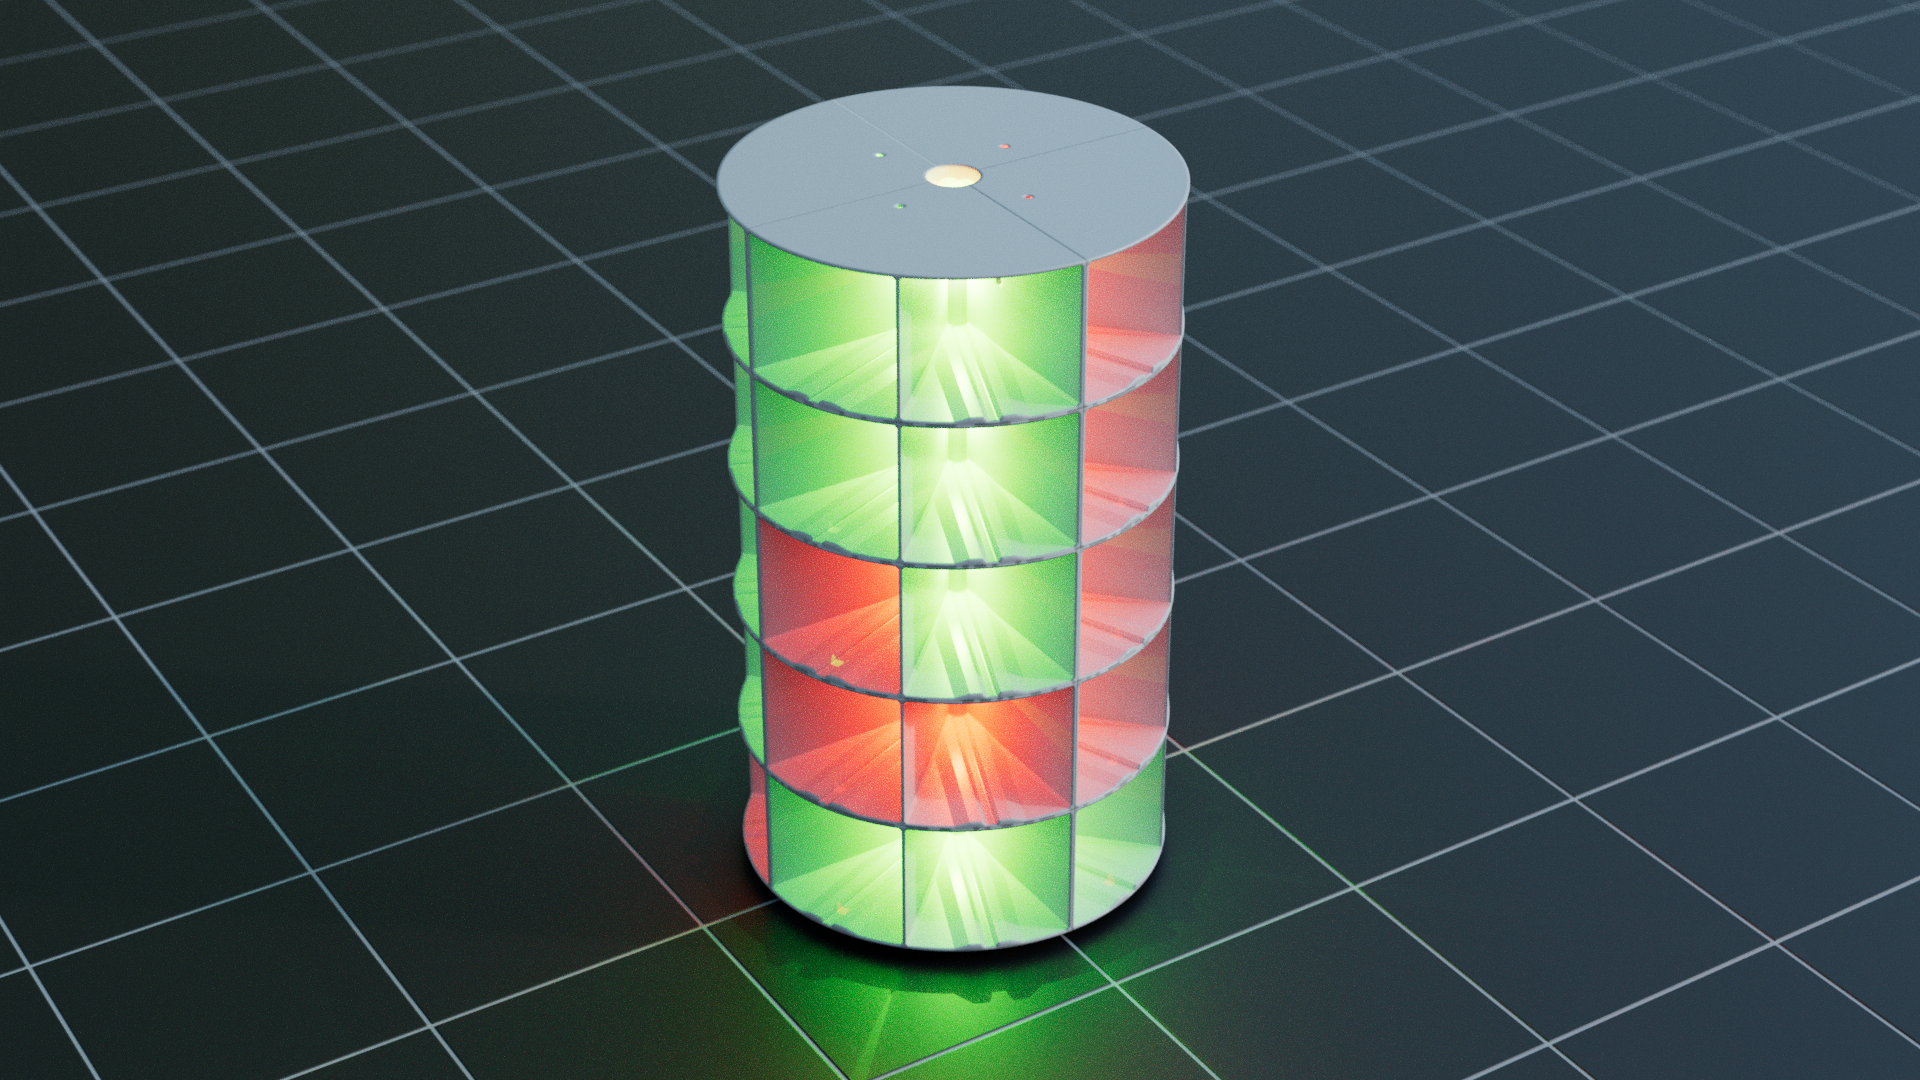
\includegraphics[width=0.8\textwidth]{images/turm_modell.png}
  \caption{Visualisierung des Modell-Turms}
  \label{fig:turm}
\end{figure}